\section{ESTRATÉGIA DE JOGO E TÉCNICAS DE CONTROLE}\label{strategy}

Para que os robôs sejam capazes de jogar, é necessário que haja estratégias de jogo, onde seja otimizada a chance de vitória dado o comportamento dos robôs. 
As decisões vão ser feitas através da analise dos dados coletados pela visão computacional, sendo assim definidas como estados da rede. 
A ação tomadas pelos robôs será feita através dos estados em que o ambiente atual do jogo vai estar. 
Esse controle pode ser feito através das técnicas de aprendizado por reforço exploradas em \cite{stone2005reinforcement} e \cite{riedmiller2009reinforcement}. 
%% Mas como os estados e ações no futebol são considerados de alta dimensão 

\subsection{Aprendizado por Reforço Profundo}

O objetivo do aprendizado por reforço profundo (Deep-RL) é controlar um agente em um ambiente na tentativa de maximizar a função de recompensa, mostrado na Figura \ref{fig:rl}.
O algoritmo da rede-Q profunda (DQN) \cite{mnih2013playing} foi capaz de ter um desempenho de nível humano em muitos dos jogos eletrônicos no Atari estimando as ações de um agente.
Contudo, enquanto a DQN pode resolver problemas em um espaço de observação complexo, ele só pode lidar com ações discretas. É possível notar que muitas tarefas, no controle de robótica, tem espaço de ações continuas.
Então a DQN não pode ser aplicada em domínios contínuos e é necessário usar um outro algoritmo capaz de lidar com esse tipo de problema.

\begin{figure}[htbp]
\centerline{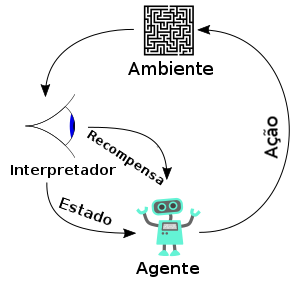
\includegraphics[width=\columnwidth]{capitulos/imagens/reinforcement_learning.png}}
\caption{Ideia principal do funcionamento do agente no Aprendizado por Reforço.}
\label{fig:rl}
\end{figure}

\subsubsection{Soft Actor-Critic (SAC)}

É um algoritmo de Deep-RL baseada na estrutura de entropia máxima para o aprendizado profundo \cite{haarnoja2017reinforcement}.
Nesta estrutura, o rede ator visa maximizar a recompensa esperada enquanto também maximizando a entropia.
Isto é, suceder em uma tarefa enquanto agindo tão aleatória como possível.
Este método é capaz de desempenhar varias atividades em aplicações de domínios contínuos \cite{haarnoja2018soft}.

\subsection{Função de Recompensa para Ataque e Defesa}

Para que a rede Deep-RL seja treinada é necessária uma função de recompensa que permita os agentes fazerem as ações que se é deseja.
Logo, é preciso formular um função de recompensa de ataque e defesa para que assim os agentes consigam jogar futebol.

As principais recompensas definidas para o jogo de futebol são as seguintes:
\begin{multline}
r (s_t, a_t) = r^{gol}_t + p^{gol}_t + c_1(d_{t-1}(b,g) - d_{t}(b,g))\\  + c_2(d_{t-1}(a,b) - d_{t}(a,b))
\end{multline}

Se a rede responsável pelas ações do agente fizer um gol uma recompensa $r^{gol}$ é dada e caso o time leve um gol uma recompensa negativa $p^{gol}$ é dada. Ambas condições representam a maiores recompensas que a rede pode receber por uma ação. 
Caso contrário, a recompensa é baseado na diferença da distância do intervalo de tempo atual com o tempo anterior $(d_{t-1}-d_t)$. Para que o agente se aproxime da bola é usado a distância do agente ao bola $d(a,b)$. Já para que a bola se aproxime do gol adversário é usado a distância da bola ao gol adversário $d(b,g)$.
%% Falta um pouquinho aqui
